% !TeX root = ../thesis.tex
\chapter{\glsxtrshort{FPGA} Model}\label{cha:fpga}
The goal of the \gls{FPGA} model is to proof the general workings of the \gls{CPU} architecture before finalizing the hardware layout and \gls{PCB} design.
With the design running on an actual \gls{FPGA} it is also possible to debug and test extension cards without the actual hardware of the \gls{EDiC}.


\section{\glsxtrshort{FPGA} Background}
An \gls{FPGA} can be seen as an intermediary between \glspl{ASIC} and general purpose \glspl{CPU}.
It allows for a lot more design flexibility in contrast to \glspl{ASIC} by being reprogrammable but at the same time has similar applications.
The first \gls{FPGA} was released by Altera in 1984 which featured a quartz window to erase the \gls{EPROM} cells that hold the configuration.
It only had eight macrocells and a maximum frequency of about 30MHz \cite{ref:altera_databook}.
Today's \glspl{FPGA} can have several million logic elements with several hundred MBs of \gls{BRAM}, more than thousand floating-point \glspl{DSP} and usual frequencies of more than 200MHz.
However, the general idea of how \glspl{FPGA} work stayed the same:

\emph{Field Programmable} means that the \gls{FPGA} can programmed in the application field, even though configure is the better word to be used.\\
\emph{Gate Array} stands for an array of logic gates which make up the \gls{FPGA}.
These logic gates can then be freely routed by the developer and with that different logic functions can be implemented.

\glspl{FPGA} are built out of so called \glspl{CLB} which can be connected with each other to create larger designs.
Such a \gls{CLB} contains several different elements like \glspl{LUT}, registers and \glspl{MUX} which allows one \gls{CLB} to provide different functionality as needed.
\begin{figure}
  \centering
  \includegraphics[width=.8\textwidth]{lut.pdf}
  \caption{Internal structure of a 2-bit \gls{LUT}}
  \label{fig:lut}
\end{figure}
Each \gls{LUT} can encode any kind of multi-bit boolean functionality.
\Cref{fig:lut} shows how a 2-bit \gls{LUT} is built out of three 2-to-1 \glspl{MUX}.
Depending on the input values of the \gls{SRAM} into the \glspl{MUX}, a different logic function can be implemented.
For example: For a \texttt{NAND} function, the \gls{SRAM} is loaded with the bits \texttt{0111}.
In \glspl{FPGA} these \glspl{LUT} usually take 4-6 bit inputs and can, therefore, implement more complex logic functions.

Combining these \glspl{LUT} with registers, complex hardware \glspl{DSP} and a lot more advanced hardware, modern \glspl{FPGA} are very capable and complex devices that are increasingly used in prototyping and low to medium quantity products.
There are several cheaply available \glspl{FPGA} development boards that are very well suited for a \gls{FPGA} prototype of the \gls{EDiC}.

\section{\glsxtrshort{FPGA} choices}
For the \gls{EDiC} the Nexys A7 development board \cite{nexysA7} with the AMD-Xilinx Artix 7 XC7A100T-1CSG324C \gls{FPGA} has been chosen.
Its synthesis tool is the AMD-Xilinx Vivado \cite{vivado} which is available as a free version and includes an advanced simulation environment.

\subsection{Language Choice}
There are two main \glspl{HDL}: Verilog and \gls{VHDL}.
Both are widely supported and used and can also be used in the same project with the help of mixed-language compilation.
At the \gls{TUB} \gls{VHDL} is taught, however, in general both are used about equally often \cite{vhdlVerilog}.
As Verilog is often cited as being less verbose and, therefore, easier to write and understand it was chosen as the hardware description language.

\begin{listing}
  \inputminted[linenos,
    breaklines,
    firstline=65,
    lastline=71,
    frame=leftline,
    xleftmargin=20pt,
  ]{verilog}{src/alu.v}
  \caption{Behavioral Verilog Description of the Adder (including XOR and AND) of the \gls{ALU} module.}
  \label{lst:alu}
\end{listing}
\Cref{lst:alu} shows the Adder described in Verilog as an example.
It iterates over all 8 bits, calculates the XOR and AND results and based on these and the carry input, the bit result and the carry output is calculated.

\subsection{Tri-state Logic in \glsxtrshortpl{FPGA}}
One major problem with tri-state bus logic for \glspl{FPGA} is that most current era \glspl{FPGA} do not feature tri-state bus drivers in the logic slices.
Most \glspl{FPGA} do have bidirectional tri-state transceiver for \gls{IO} but not for internal logic routing.
However, the \glspl{HDL} (both \gls{VHDL} and Verilog) support tri-state logic and the Xilinx Simulation tool also does.
Therefore, a simulation with tri-state logic would work but it cannot be synthesized.

\begin{figure}[t]
  \centering
  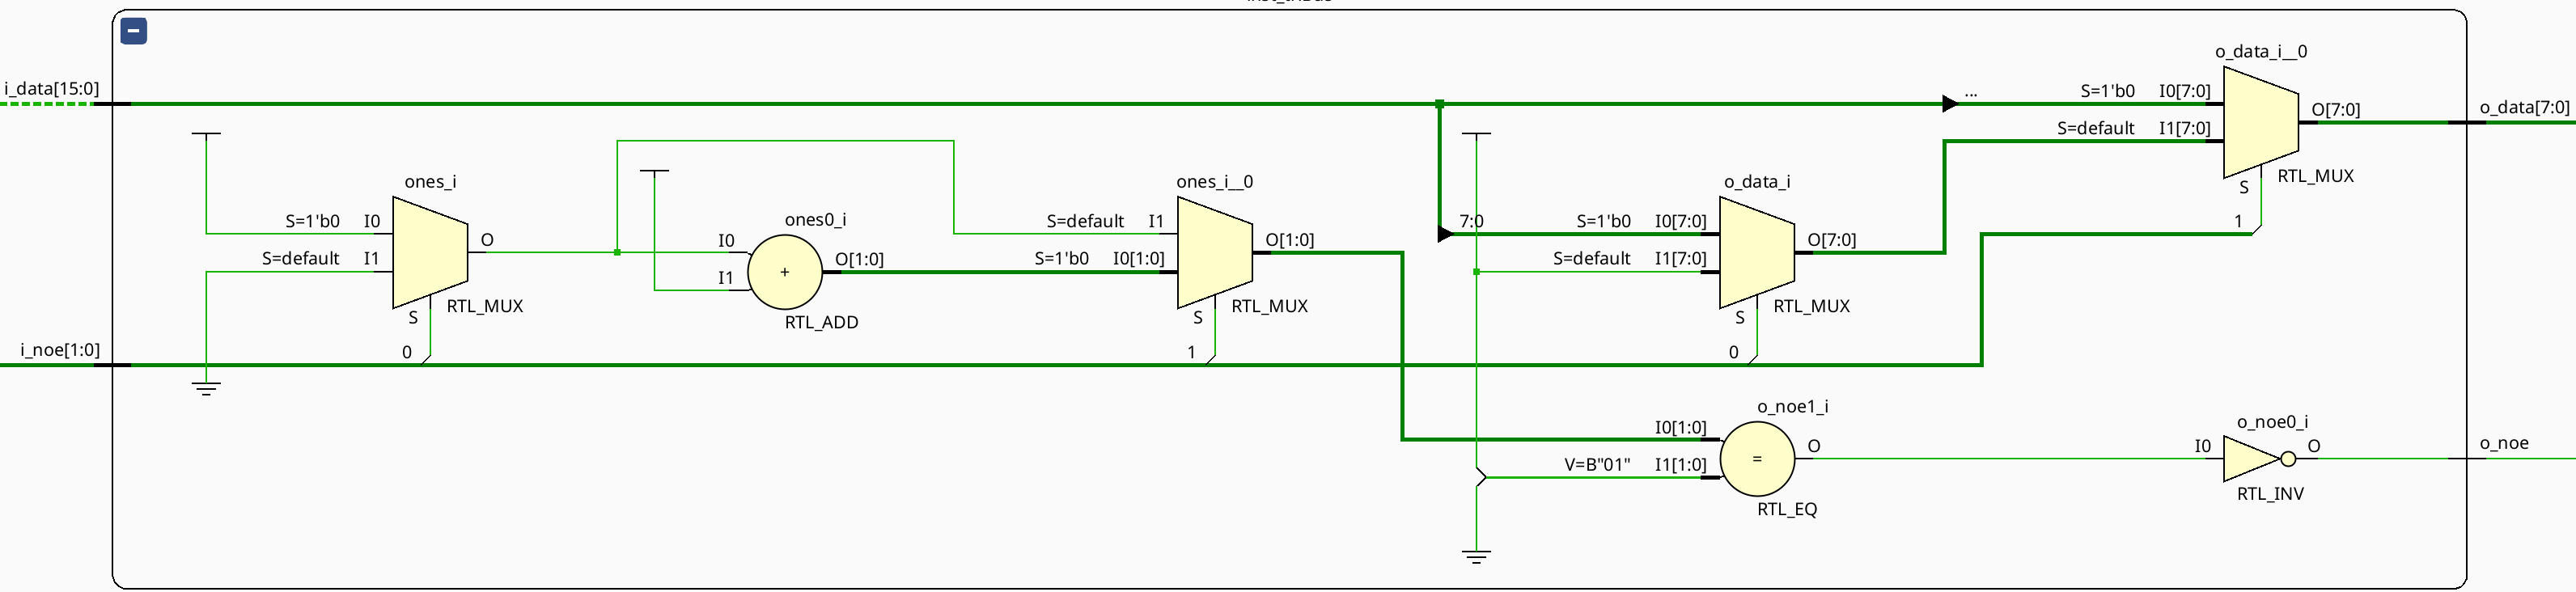
\includegraphics[width=\textwidth]{tristatenet.png}
  \caption{The elaborated tri-state module with two 8 bit inputs.}
  \label{fig:tristatenet}
\end{figure}
This is solved with a custom module for each tri-state network ``tristatenet.v''.
Each tri-state driver exposes the current data and output enable signal to the tristate module which then has only one output which represents the value of the net.
If none of the driver have an active output enable, the output is \texttt{0xff}; if one of the driver has an active output enable, the output represents its value and if more than one driver have an active output enable, an error is raised.
The modules logic representation for a tri-state net with two inputs is shown in \cref{fig:tristatenet}.
The \texttt{o\_noe} is only active (low) if exactly one input \texttt{i\_noe} is active (low) and depending on it, the data output is selected.
For this \gls{FPGA} it is implemented with one \texttt{LUT4} primitive per output data bit.

\section{Behavioral Implementation}
Two kinds of \gls{FPGA} designs were developed in the process.
The first is a behavioral description of the whole \gls{CPU} and, therefore, only models the general workings of a module but does not describe the individual chips that are used in the final hardware assembly.
The description in \cref{lst:alu}, for example, is a behavioral description because it only describes the logical level of what should happen.
This is quite useful for development, because it is quickly changed and bugs are fixed more efficiently as opposed to a chip-level model.

To visualize how a behavioral simulation looks like, a simulation of the code in \cref{lst:add_wave} is shown in \cref{fig:add_wave}.
The first instruction (\mintinline{ARM}{mov r1, 0x12}) starts at \qty{1}{\micro\second} where the instruction step counter is 0 and the instruction fetch is executed.
Step 1 increments the program counter and starts the instruction decoding.
The \mintinline{ARM}{mov} instruction only consists of one step and, therefore, the \texttt{ctrInstrFinishedN} signal is asserted in step 2 together with the control signals of the actual instruction.
Due to \texttt{ctrInstrFinishedN}, the step counter is reset to 0 and the second instruction (\texttt{pc==1}) is executed.
After the instruction fetch steps, the \gls{ALU} adds \texttt{0x12} and \texttt{0x42} at \qty{2}{\micro\second} and writes the result into \texttt{r1} at \texttt{step==3}.
The third instruction then just branches to itself, resulting in an infinite loop.
\begin{sidewaysfigure}[p]
  \centering
  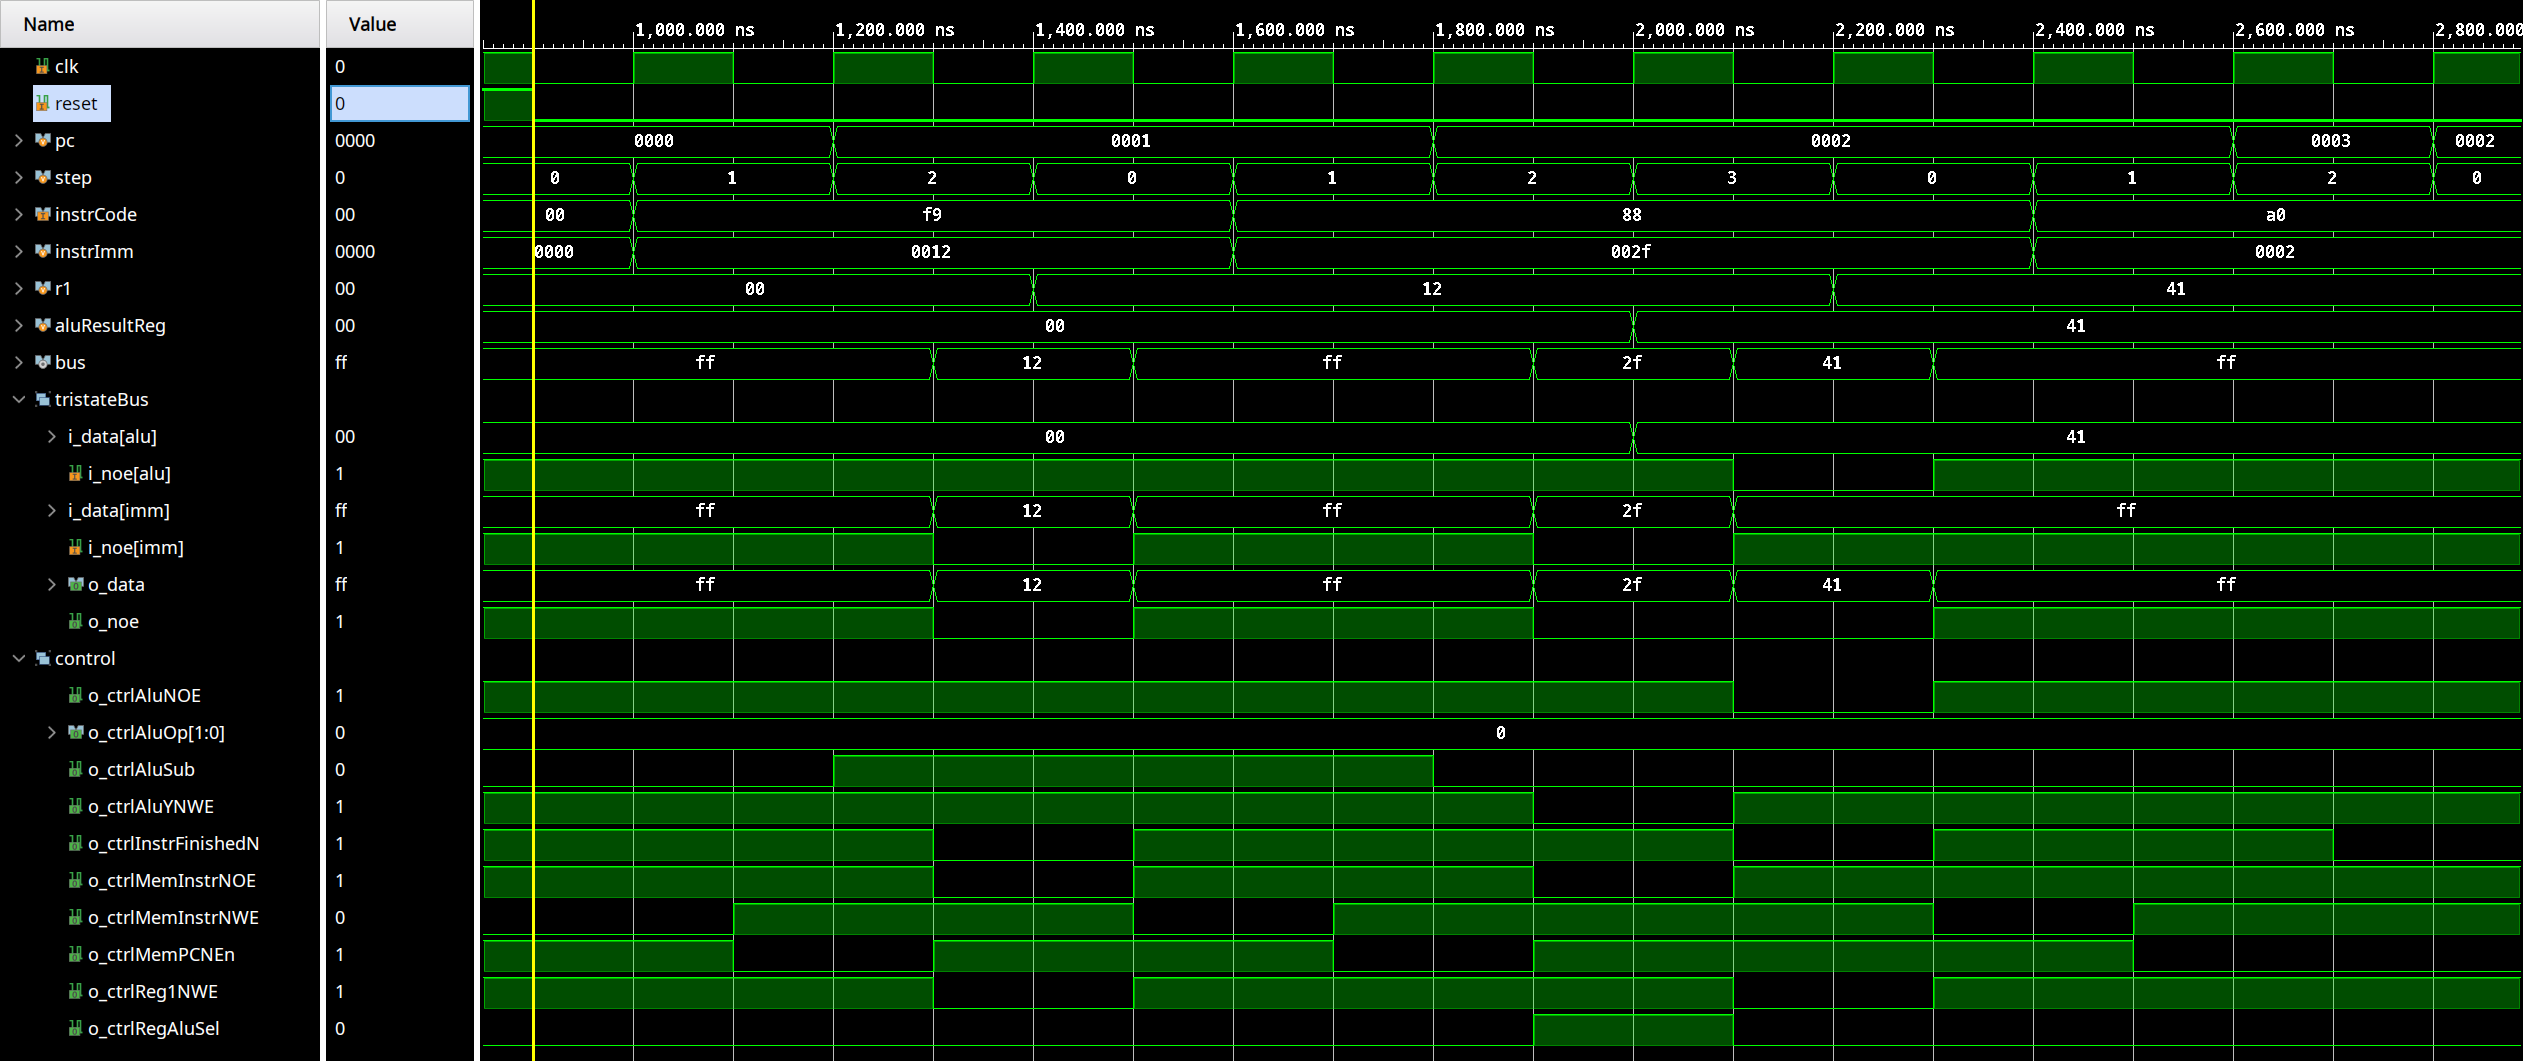
\includegraphics[width=\textwidth]{behav_add_wave.png}
  \caption{Waveform of the relevant signals for setting a register to \texttt{0x12} and adding \texttt{0x2f} to it (Assembler code is shown in \cref{lst:add_wave}).}
  \label{fig:add_wave}
\end{sidewaysfigure}
\begin{listing}
  \inputminted[linenos,
    breaklines,
    frame=leftline,
    xleftmargin=20pt,
  ]{ARM}{src/sim_test.s}
  \caption{The code for the waveform example of \cref{fig:add_wave}.}
  \label{lst:add_wave}
\end{listing}

\section{Chip-level Implementation}
With the behavioral simulation working, the hardware schematic can be developed.
The schematic and then the placing and routing for the \gls{PCB} is described in \cref{cha:hardware}.
However, for the \gls{EDiC} it was decided to add another verification step after developing the schematic.
From the schematic a netlist is generated which is usually used to summarize all the components and connections in a machine readable format for the software that does placing and routing.
Here, a tool was written which converts a given netlist into a Verilog file which can be compiled and synthesized by Vivado.
\subsection{Conversation Script}
\begin{listing}
  \inputminted[linenos,
    breaklines,
    frame=leftline,
    xleftmargin=20pt,
  ]{clojure}{src/edifInstance.edn}
  \caption{An \glsxtrshort{EDIF} definition of an instance as exported by OrCAD/CAPTURE.}
  \label{lst:edifInstance}
\end{listing}
\begin{listing}
  \inputminted[linenos,
    breaklines,
    frame=leftline,
    xleftmargin=20pt,
  ]{clojure}{src/edifNet.edn}
  \caption{An \glsxtrshort{EDIF} definition of a net as exported by OrCAD/CAPTURE.}
  \label{lst:edifNet}
\end{listing}
The netlist file used is an \texttt{*.edn} which is exported by OrCAD/CAPTURE version 9.2.1.148.
It follows the \gls{EDIF} and contains a list of all instances (i.e. \glspl{IC} and other components) with port numbers and a second list of all nets (connections between ports).
The conversion script consists of a parser which analyzes such a netlist.
The parsed netlist is then further processed until a verilog file can be created.
The generated verilog file only consists of wire definitions and module instantiations.
Each of the instantiated modules has its own, manually written implementation.
The implementation for an \texttt{74F08} (quad AND gate) is, for example, shown in \cref{lst:74x08}.
\begin{listing}[t]
  \inputminted[linenos,
    breaklines,
    frame=leftline,
    xleftmargin=20pt,
  ]{Verilog}{src/ic74x08.v}
  \caption{Verilog implementation for the 74F08 \gls{IC}.}
  \label{lst:74x08}
\end{listing}

\Cref{lst:edifInstance} specifies the instance U54 which is an \texttt{74AS867}.
The format also specifies the port numbers but they are not processed by the parser because they are not required.
\Cref{lst:edifNet} then specifies a net with the name \texttt{PCIN0} which connects U52 port 18 with U51 port 18 and U54 port 3.
In this case U52 and U51 are both \texttt{74F245} octal bus transceivers where port 18 is the B0 tri-state output port and U54 is a \texttt{74AS867} (synchronous up/down counter with load) where port 3 is the D0 input port.
Depending on the control signals of U51 and U52 this net connects the 0th bit of the bus or the instruction immediate with the 0th bit of the load input of the \gls{PC}.
Internally the list of instances and list of nets is combined into a list of instances where each instance contains a mapping of port numbers to connected nets.

The parser discards all components except logic \glspl{IC} (id starting with `U') and \qty{0}{\ohm} resistors.
The schematic includes some \qty{0}{\ohm} resistors between control signals to be able to rewire them more easily on the \gls{PCB} if needed.
As they essentially behave as direct connections, the nets on either side of one \qty{0}{\ohm} resistor are merged.

The basic instances are easily converted to verilog instantiations.
However, there are some obstacles that need to be taken with more advanced instances.
\subsubsection{\glsxtrshort{EEPROM}}
\begin{listing}[t]
  \inputminted[linenos,
    breaklines,
    firstline=1364,
    lastline=1368,
    frame=leftline,
    xleftmargin=20pt,
  ]{Verilog}{src/generated.v}
  \caption{Verilog instantiation of the microcode ROM generated out of three \gls{EEPROM} instantiations.}
  \label{lst:rom_inst}
\end{listing}
The 6 \glspl{EEPROM} (3 for the instructionROM and 3 for the microcode) need to be instantiated with the correct data loaded into them.
Those six instantiations are identified by the unit id and the wires are then connected to one of the custom Xilinx ROM IP Cores which are configured with the respective initial values.
The addresses for one ROM instantiations are used and then all 24 data ports from the 3 \glspl{EEPROM} are connected resulting in a verilog instantiation as shown in \cref{lst:rom_inst}.
\subsubsection{tri-state Ports}
\begin{listing}[t]
  \inputminted[linenos,
    breaklines,
    firstline=1794,
    lastline=1801,
    frame=leftline,
    xleftmargin=20pt,
  ]{Verilog}{src/generated.v}
\caption{Verilog instantiation for the tri-state Net \texttt{PCIN0}.}
  \label{lst:tristate_inst}
\end{listing}
Some \glspl{IC} provide tri-state ports.
As discussed above, they cannot be implemented on \glspl{FPGA} and, therefore, need to be converted.
The same tristatenet component as in the behavioral implementation is used.
However, for this to work, each bidirectional port of the \glspl{IC} needs to be replaced by one input and one output port.
Also, one output enable port needs to be added.
Then the output port that replaced the bidirectional port is connected to an input of the tristatenet instance and a new net is created for each tristatenet which is the actual value of the net (the output of the tristatenet module).
The tristatenet for the \texttt{PCIN0} signal (\cref{lst:edifNet}) is represented by the instantiation shown in \cref{lst:tristate_inst}.

\subsubsection{\glsxtrshort{RAM} and \glsxtrshort{EEPROM} clock}
Another problem with the \gls{FPGA} implementation in general is that both, the \gls{SRAM} and \gls{EEPROM} chips used are asynchronous and the \gls{FPGA} only has synchronous logic elements.
In the behavioral implementation, exact timings were no requirement and, therefore, the memory and \glspl{ROM} were clocked with the inverse clock, mimicking an asynchronous behavior.
However, for the exact netlist \gls{FPGA} implementation this is not a good way to mimic the behavior.
Therefore, the exact delay of both chips were calculated with the help of the datasheets and they are both clocked with a custom clock that is out of phase with the global logic clock by the exact amount of the delay.
\begin{figure}
  \centering
  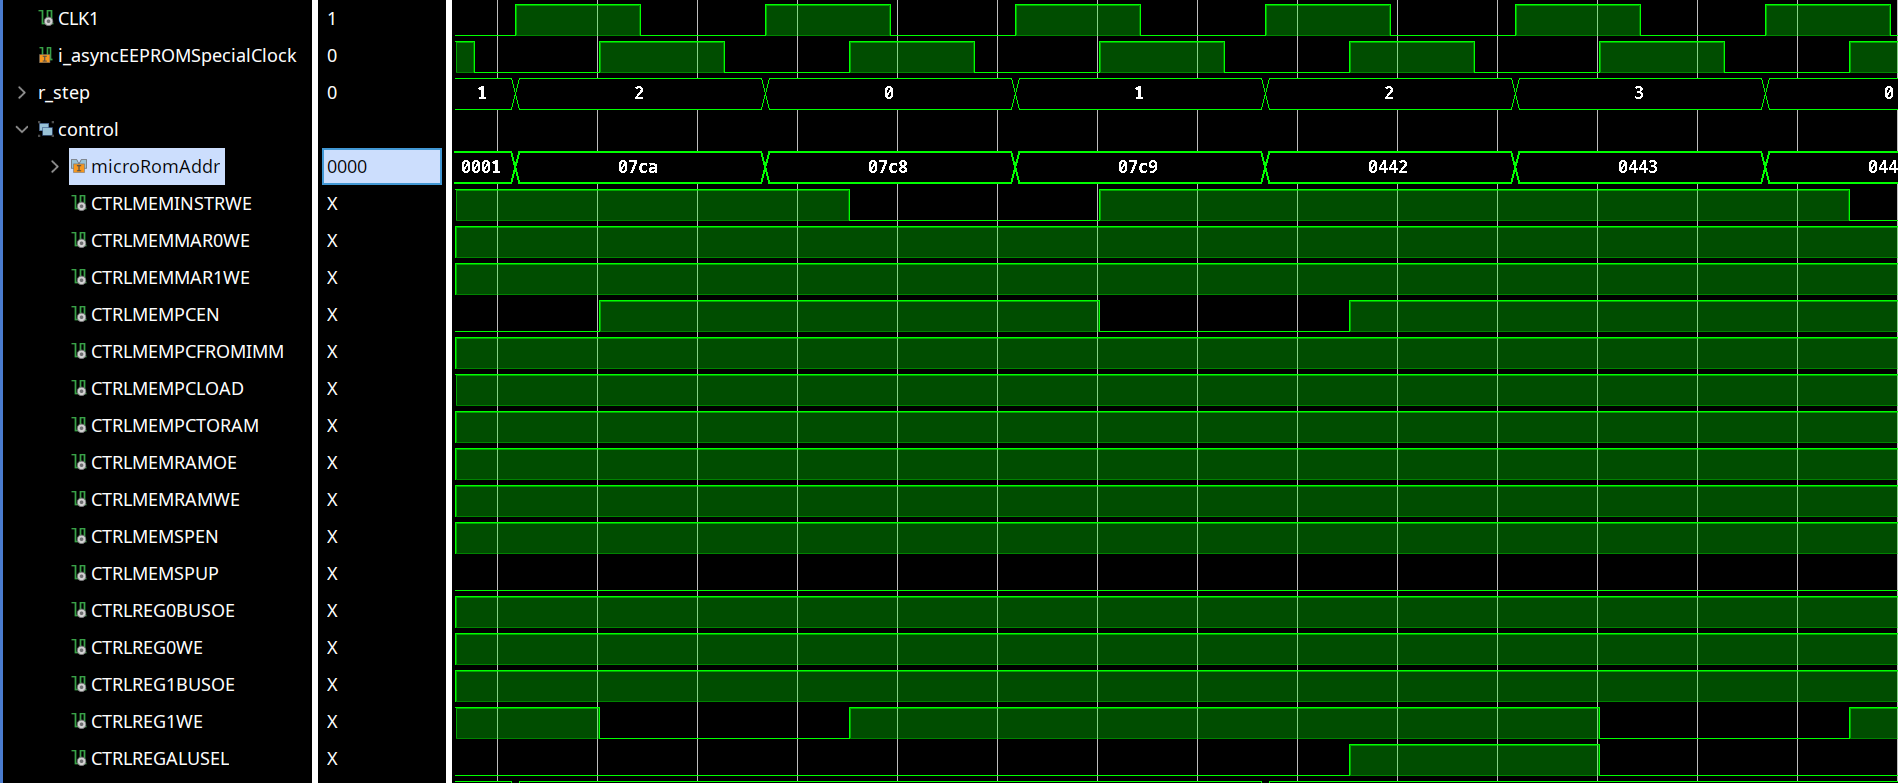
\includegraphics[width=\textwidth]{asyncClockWave.png}
  \caption{Waveform showing the clock used for the \gls{FPGA} \gls{ROM} to mimic the asynchronous behavior of the \glspl{EEPROM}.}
  \label{fig:asyncClockWave}
\end{figure}

This means, that the clock inputs of the memory and \gls{EEPROM} instantiations are replaced with the corresponding custom clock as can be seen in \cref{lst:rom_inst}.

\Cref{fig:asyncClockWave} visualizes how the main clock (\texttt{CLK1} in the waveform) and the clock for the \gls{ROM} (\texttt{asyncEEPROMSpecialClock} in the waveform) differ in phase.
Consequently, the step register and with it the address for the microcode \gls{ROM} change with a rising edge of the main clock but all the control signals which are outputs of the \gls{ROM} change with the rising edge of the phase shifted clock.

\subsubsection{Assignments}
There are some connections which are unique to the \gls{FPGA} implementation and, therefore, are not contained in the netlist.
These are mainly the inputs and outputs of the \gls{CPU} for the \gls{IO} extensions, the user buttons (reset, step etc.), clock oscillator, breakpoint addresses and so on.
However, one exception are the \texttt{L1-L4} and \texttt{H1-H4} nets which are static nets connected to ground or 5V through resistors.
They are used for logic inputs of \glspl{IC} instead of directly using GND or 5V to ease the error fixing on the \gls{PCB}.
If one would connect the pins directly to the GND or 5V planes, it would be hard to heat up the solder on the pin for removal because the whole plane needs to be heated.
Additionally, when connected to the plane, there is no trace that can be scratched through if the pin needs to be connected to another net.

In the \gls{FPGA} design the nets \texttt{L1-L4} and \texttt{H1-H4} are, therefore, assigned to 0 or 1 respectively.

\subsubsection{Display Driver}
\begin{figure}
  \centering
  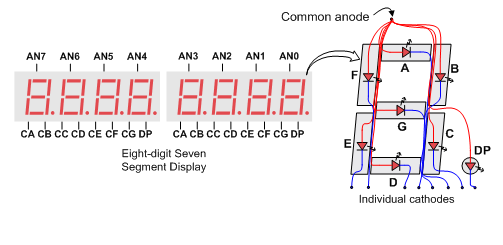
\includegraphics[width=.8\textwidth]{7segmentNexysA7.png}
  \caption{Overview of the 8 7-segment displays of the Nexys A7 development board \cite{7segNexys}.}
  \label{fig:7segNexys}
\end{figure}
The hardware build will feature 2 displays for the built-in \gls{IO} which can be directly addressed with 4 bits to display hexadecimal digits.
The \gls{FPGA} development board on the other hand, features simpler and more common 7-segment displays.
In total, there are 8 7-segment displays of which two are used as the built-in \gls{IO} and the others are used for debugging when the \gls{CPU} is halted.
The wiring of the displays is shown in \cref{fig:7segNexys}.
For this purpose, a custom displayDriver has been developed which has 8 four bit data inputs for the digits plus 8 inputs for the dots between the digits.
Additionally, 8 bits encode which 7-segment displays should be illuminated.
It loops through the digits by setting each anode to 0 individually and setting the cathodes according the corresponding input bits.
This way, each display is illuminated for 2ms which makes it look like all displays are illuminated all the time.

\subsection{RS232 \gls{IO} Extension Debugging}
\begin{sidewaysfigure}[p]
  \centering
  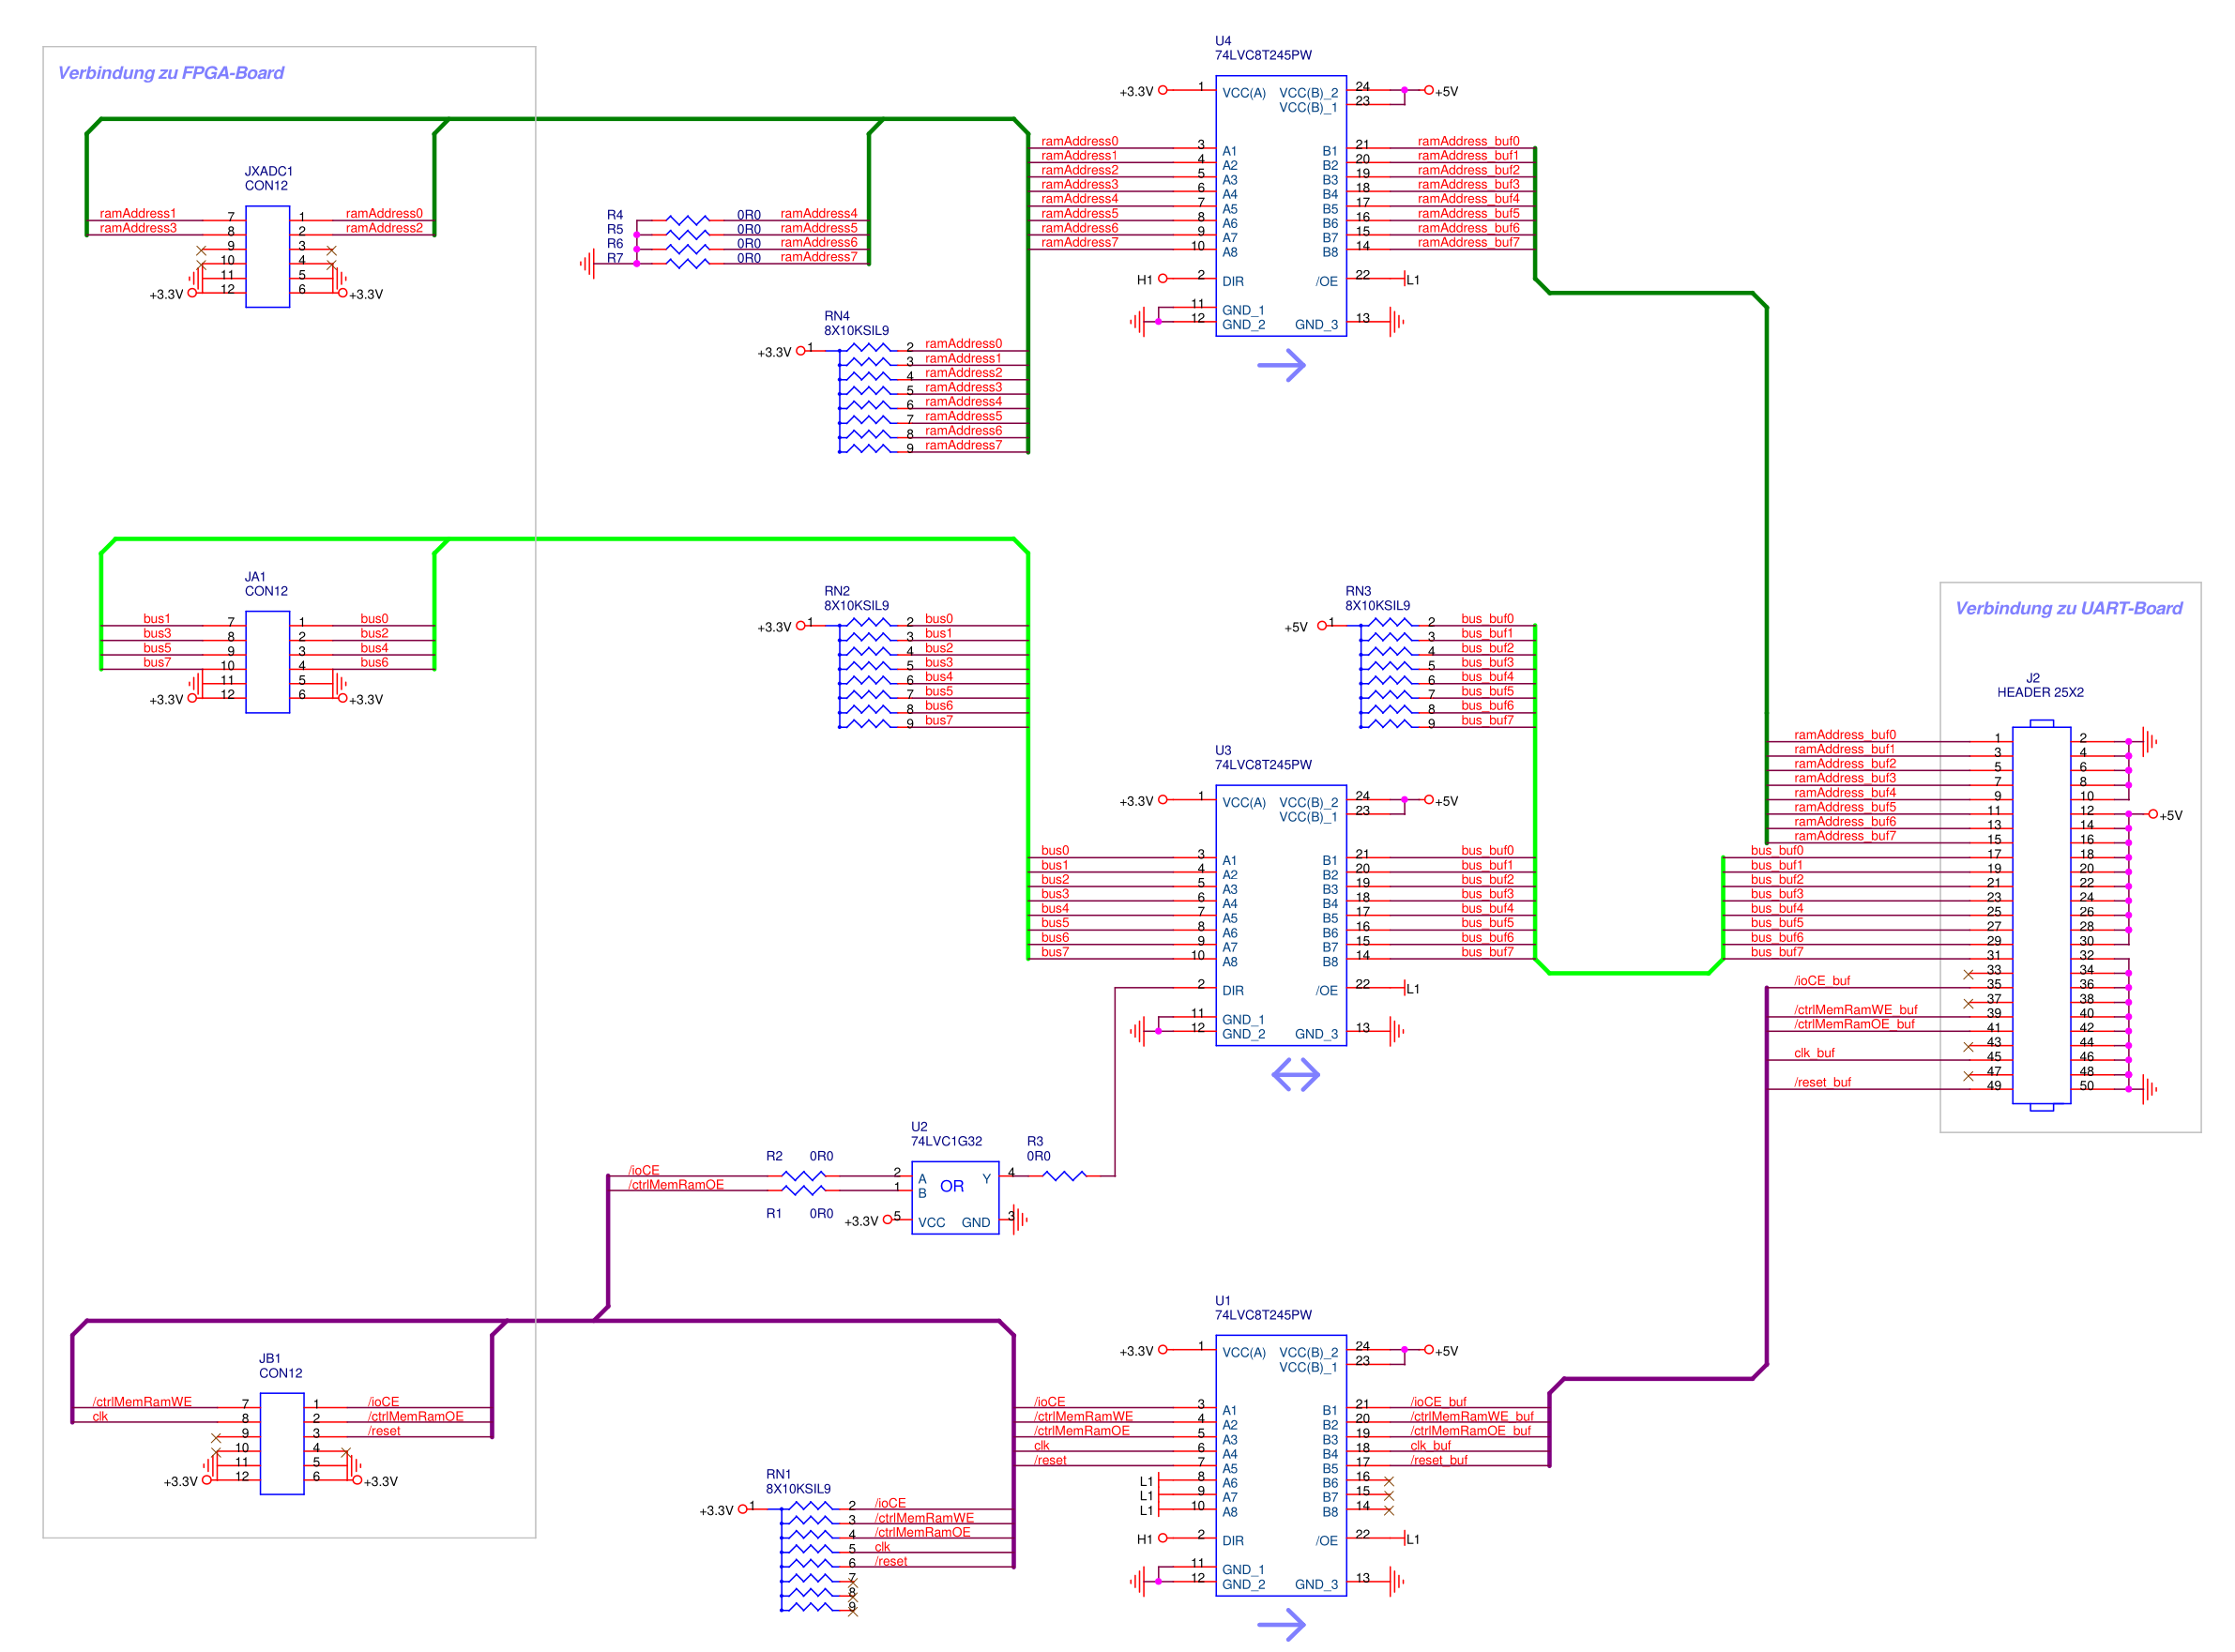
\includegraphics[width=\textwidth]{uartTestSch.png}
  \caption{The Schematic for the 3V3 to 5V conversion to use extension cards with the \gls{FPGA} development board.}
  \label{fig:3v3to5vSch}
\end{sidewaysfigure}
One goal of creating a logical replication of the \gls{CPU} on a \gls{FPGA} was to verify the \gls{IO} extension cards before ordering the large \gls{PCB} for the \gls{CPU}.
All extension cards will be daughterboards and sit on top of the main \gls{PCB} in a smaller form factor.
The following logical connections are passed through pin headers:
\begin{itemize}
  \item Bus (8 bits, bidirectional)
  \item \gls{IO} Address (lower 8 bits, to \gls{IO})
  \item Control Signals:
  \begin{itemize}
    \item \texttt{\textoverline{ioCE}}: active when the upper 8 \gls{RAM} address bits equal \texttt{0xfe}.
    \item \texttt{\textoverline{ctrlMemRamWE}}: write enable signal. Write should only happen when \texttt{\textoverline{ioCE}} is active.
    \item \texttt{\textoverline{ctrlMemRamOE}}: output enable signal. Read should only happen when \texttt{\textoverline{ioCE}} is active.
    \item \texttt{clk}: Clock signal.
    \item \texttt{\textoverline{reset}}: Reset signal.
  \end{itemize}
\end{itemize}
Additionally, ground and 5V is passed through the connector.
However, the Nexys A7 \gls{FPGA} development board only features digital 3V3 connections on the side.
Thus, an adapter board is required which converts the 3V3 voltages to 5V and the other way around while providing the correct pin locations for the Nexys A7 board and the daughterboard.
Its schematic is shown in \cref{fig:3v3to5vSch} where the \texttt{74LVC8T245} is used as a voltage converting buffer.
For the control signals and addresses, its direction is always from the A port (3V3) to the B port.
On the other hand, the direction pin of the bus buffer is low (from B to A) when both, output enable and chip enable, signals are active.